\chapter{Linguagem}
\label{lang}

O usuário se comunica com a interface através de um texto, chamado de programa,
que contém os objetos de interesse. 
Por exemplo, em GeoGebra, o círculo unitário pode ser
definido como
\texttt{c = Curve(cos(t), sin(t), t, 0, 2pi)}.
Na linguagem desse projeto, a definição seria
\texttt{curve c(t) = (cos(t), sin(t), 0), t : [0, 2pi];}.

O código \ref{ex1} é um exemplo.
\begin{lstlisting}[caption=Exemplo de objetos,label=ex1]
#circle and tangents
param r : [/2, 1];
param o : [0, 2pi];
curve c(t) = r(cost, sint, 0), t : [0, 2pi];
grid k : [0, 2pi, 8];
define k2 = k + o;
point p = ck2;
vector v = c'k2 @ p;

#function and surface
#function f(x, y) = x^2+y^2;
#surface s(u,v) = (u,v,f(u,v)), u : [-1, 1], v : [-1, 1];
\end{lstlisting}

A linguagem permite comentários no estilo da linguagem Python, usando \texttt{\#}.

O programa declara os seguintes objetos:

\begin{table}[ht]
\caption{Tipos de objeto}
\label{objtypes}
\begin{centering}
\begin{tabularx}{\textwidth}{||c|X||}
    \hline
    \texttt{r} e \texttt{o} & parâmetros que podem ser alterados na interface.
    Seus valores devem estar nos intervalos indicados. \\ 

    \hline
    \texttt{c} & uma curva parametrizada por \texttt{t}.
    O domínio da parametrização é o intervalo indicado.
    A curva depende do parâmetro \texttt{r}, que foi definido anteriormente. \\

    \hline
    \texttt{k} & uma grade de 8 pontos igualmente espaçados no intervalo indicado.
    Uma grade é tratada como uma constante, assim como um parâmetro.
    Se um objeto desenhável depende de uma grade, uma instância é desenhada para cada valor da grade.
    Um objeto pode depender de mais de uma grade. \\

    \hline
    \texttt{k2} & uma constante, e não pode ser alterada na interface como os parâmetros.
    Esse tipo de objeto pode ser usado para deixar o programa mais legível. \\
    
    \hline
    \texttt{p} & o ponto da curva \texttt{c} de parâmetro \texttt{t = k2}.
    Esse objeto depende indiretamente de \texttt{k}, então é instanciado 8 vezes. \\
    
    \hline
    \texttt{v} & o vetor tangente da curva \texttt{c} no ponto \texttt{p} 
    e desenhado a partir do mesmo ponto.
    O vetor também depende indiretamente de \texttt{k}, então é desenhado 8 vezes. \\
    \hline
\end{tabularx}
\end{centering}
\end{table}

A figura \ref{img:ex1} demonstra os objetos declarados em perspectiva 3D.
\begin{figure}[!ht]
    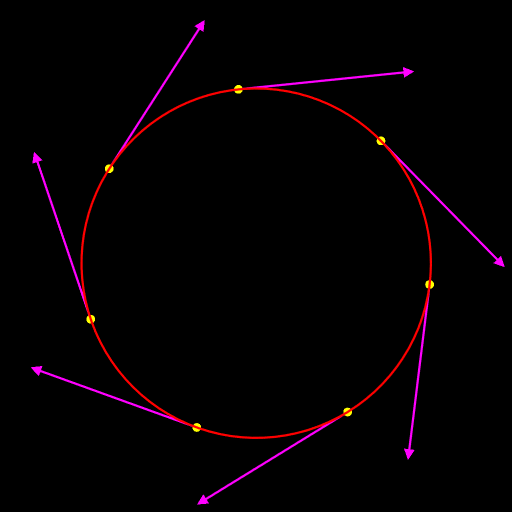
\includegraphics[width=\linewidth]{ex1.png}
    \caption{Exemplo 1}
    \label{img:ex1}
\end{figure}

Os objetos \texttt{f} e \texttt{s} estão comentados, então não são considerados.
Estão presentes apenas para o exemplo ter todos os tipos de objeto.

A linguagem de descrição de objetos não é trivial, nem sua sintaxe matemática,
que possui elementos inventados para esse projeto.
A seguir, uma breve lista de observações:

\begin{itemize}
\item
Os objetos desenháveis são pontos, vetores, curvas e superfícies.
Pontos e vetores podem ser usados em outros objetos, sendo tratados como tuplas.
Por exemplo, \texttt{v} usa o ponto \texttt{p}.
Curvas e superfícies podem ser usadas como funções, mas sem a restrição no domínio.
Por exemplo, \texttt{p} usa \texttt{c} como função.
Um objeto só pode se referir aos objetos definidos anteriormente.
Os parâmetros das curvas e superfícies podem ter qualquer nome disponível.

\item
Há duas constantes pré-definidas: \texttt{pi} e \texttt{e};
e diversas funções pré-definidas:
\texttt{sin}, \texttt{cos}, \texttt{tan},
\texttt{exp}, \texttt{log}, \texttt{sqrt} e \texttt{id}.
A função \texttt{id} é a identidade é útil apenas no funcionamento interno do sistema.

\item
Parâmetros e grades podem ser multidimensionais:
\texttt{param T : [0, 1], [0, 1];}. Assim, o objeto \texttt{T} é uma tupla,
e seus elementos podem ser obtidos com \texttt{T\_1} e \texttt{T\_2}.

\item As grades das curvas e superfícies são por padrão 100 e 100x100, respectivamente.
É possível alterar esse valor informando um intervalo do
tipo grade: \texttt{[0, 2pi, 250]}.

\item
Há 4 operadores unários. Os operadores \texttt{+} e \texttt{-} são os usuais.
A operação \texttt{*x} representa \texttt{xx}, e \texttt{/x} é igual a \texttt{1/x}.
Para números reais, multiplicação com \texttt{*} e por justaposição são equivalentes.
Porém, para tuplas, \texttt{a*b} representa o produto vetorial
e \texttt{ab} representa o produto escalar.
Assim, \texttt{*x} calcula o quadrado do módulo do vetor \texttt{x}.
Uma função que normaliza vetores pode ser
definida assim: \texttt{function N(x) = x/sqrt*x;}.

\item
Numa aplicação de função de uma variável, o argumento não precisa de parênteses:
\texttt{sin x}.
O argumento pode ter operadores unários e até expoentes:
\texttt{sin -x\textasciicircum2 = sin(-x\textasciicircum2)}.
Deve-se tomar cuidado com expoentes:
\texttt{sin(x)\textasciicircum y = sin(x\textasciicircum y)}.
Para a exponenciação de uma aplicação,
deve-se usar a sintaxe: \texttt{sin\textasciicircum2 x}.

\item
Não é sempre necessário uma separação entre identificadores.
Por exemplo, considere \texttt{sinx}.
Caso haja um termo chamado \texttt{sinx} definido, esse seria o
identificador reconhecido.
Caso contrário, \texttt{sin x} será reconhecido,
mesmo que \texttt{sinx} seja definido posteriormente
(\texttt{sinx} seria reconhecido apenas depois de sua definição).
Em geral, o maior identificador definido será reconhecido.
\end{itemize}

O código \ref{ex2} é outro exemplo.
\begin{lstlisting}[caption=Exemplo de objetos,label=ex2]
#sphere and coordinates
function f(u,v) = 
    (sin(piv)cos(2piu), sin(piv)sin(2piu), cos(piv));

param U : [0, 1];
param V : [0, 1];
point p = f(U,V);

curve cu(t) = f(t, V), t : [0, 1];
curve cv(t) = f(U, t), t : [0, 1];

function N(x) = x/sqrt*x;
vector vu = Nf_u(U,V) @ p;
vector vv = Nf_v(U,V) @ p;

surface s(u,v) = f(u,v)*0.99, u : [0, 1], v : [0, 1];
\end{lstlisting}

A figura \ref{img:ex2} demonstra o programa em perspectiva 3D.
\begin{figure}[!ht]
    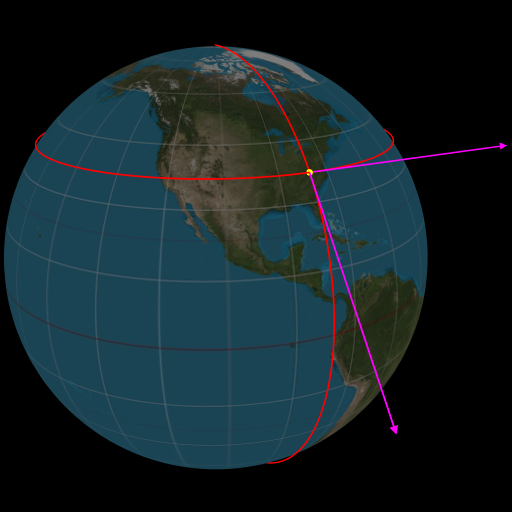
\includegraphics[width=\linewidth]{ex2.png}
    \caption{Exemplo 2 - Perspectiva em 3D}
    \label{img:ex2}
\end{figure}

A figura \ref{img:ex2gt} demonstra o geodesic tracing.
\begin{figure}[!ht]
    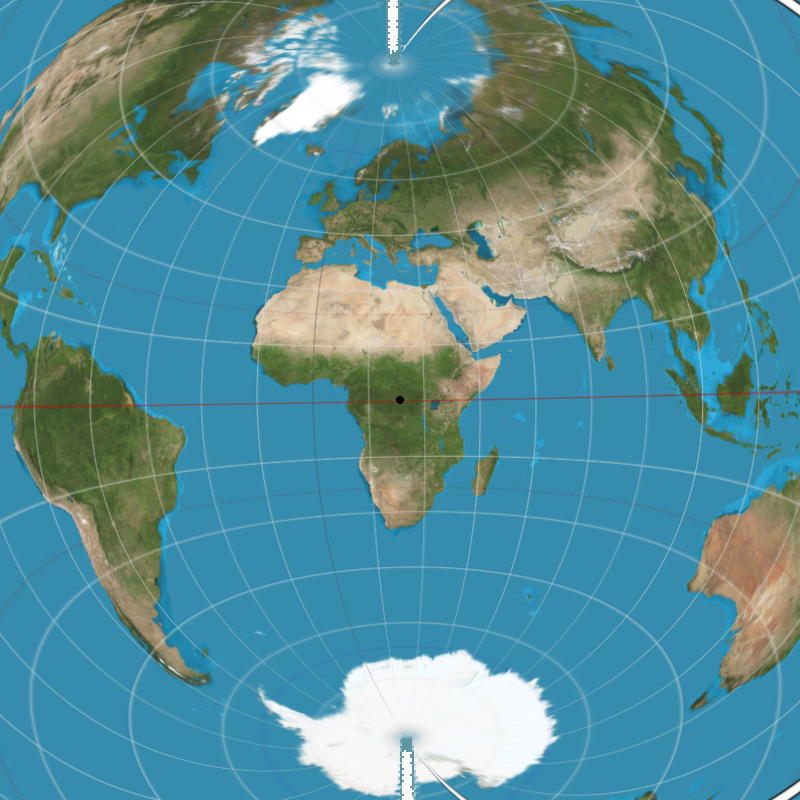
\includegraphics[width=\linewidth]{ex2gt.png}
    \caption{Exemplo 2 - geodesic tracing}
    \label{img:ex2gt}
\end{figure}